% ch2p21_004: Adding text
% to karl's activity
\documentclass[tikz, border=10pt]{standalone}

\usepackage{tikz}
\usetikzlibrary{intersections}

\begin{document}
	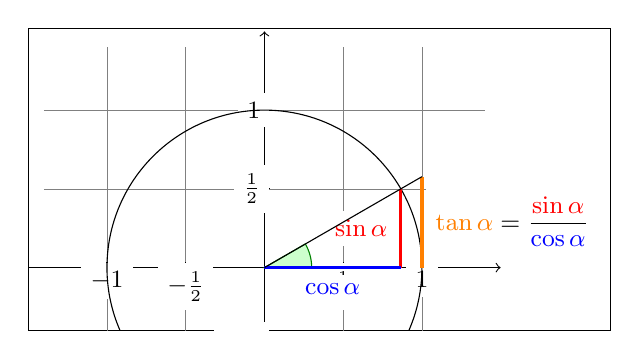
\begin{tikzpicture}[scale=2]
		\clip[draw] (-1.5, -0.4) rectangle (2.2, 1.52);
		
		\draw[step=0.5cm, gray, very thin] (-1.4, -1.4) grid (1.4, 1.4);
		\draw[->] (-1.5, 0) -- (1.5, 0); % x-axis
		\draw[->] (0, -1.5) -- (0, 1.5); % y-axis
		
		\foreach \x/\xtext in {-1, -0.5/-\frac{1}{2}, 0.5/\frac{1}{2}, 1}
		\draw (\x cm, -1pt) -- (\x cm, 1pt) node[anchor=north, fill=white] {\small $\xtext$};
		\foreach \y/\ytext in {-1, -0.5/-\frac{1}{2}, 0.5/\frac{1}{2}, 1}
		\draw (-1pt, \y cm) -- (1pt, \y cm) node[anchor=east, fill=white] {\small $\ytext$};
		
		\draw (0, 0) circle [radius=1cm];
		
		\filldraw[fill=green!20, draw=green!50!black] (0, 0) -- (3mm, 0mm)
		arc [start angle=0, end angle=30, radius=3mm] -- cycle;
		
		% Sine line
		\draw[red, very thick] (30:1cm) -- node [left=1pt, fill=white] {\small $\sin \alpha$} +(0, -0.5);
		% Cosine line
		\draw[blue, very thick] (30:1cm) ++(0, -0.5) -- node [below=2pt, fill=white] {\small $\cos \alpha$} (0, 0);
		
		% \path without draw or fill option is not displayed.
		\path [name path=upward line] (1, 0) -- (1,1);
		\path [name path=sloped line] (0, 0) -- (30:1.5cm);    % a bit longer, so that there is an intersection
		
		% Tan line
		% (add `\usetikzlibrary{intersections}` after loading tikz in the preamble)
		\draw [name intersections={of=upward line and sloped line, by=newCoordinates}]
			[very thick, orange] (1, 0) -- node [right=1pt, fill=white] {\small $\displaystyle \tan \alpha \color{black} = \frac{\color{red}\sin \alpha}{\color{blue}\cos \alpha}$} (newCoordinates);
			
		% Line from origin to tan line
		\draw (0, 0) -- (newCoordinates);
		
	\end{tikzpicture}
\end{document}